\section{Observation model}
\label{sec:observationModel}
Figure \ref{fig:observModel} shows the classification of continuous and discrete data models in \pml \currpml. 
The defining characteristic of data is their distribution which will be described first
\begin{itemize}
\item
Continuous data
\begin{itemize}
\item
usually described by the normal distribution.
\end{itemize}
\item
Discrete data
\begin{itemize}
\item
Count data -- non-negative integers -- described by the Poisson or a related distribution.
\item
Categorical data -- finite set of integer values, nominal or ordered -- described by the Bernoulli
or the categorical distribution. 
\item
Time-to-event data -- time until an event occurs, can be unique or repeated -- described by 
survival or hazard function.
\end{itemize}
\end{itemize}

\begin{figure}[h!]
\centering
 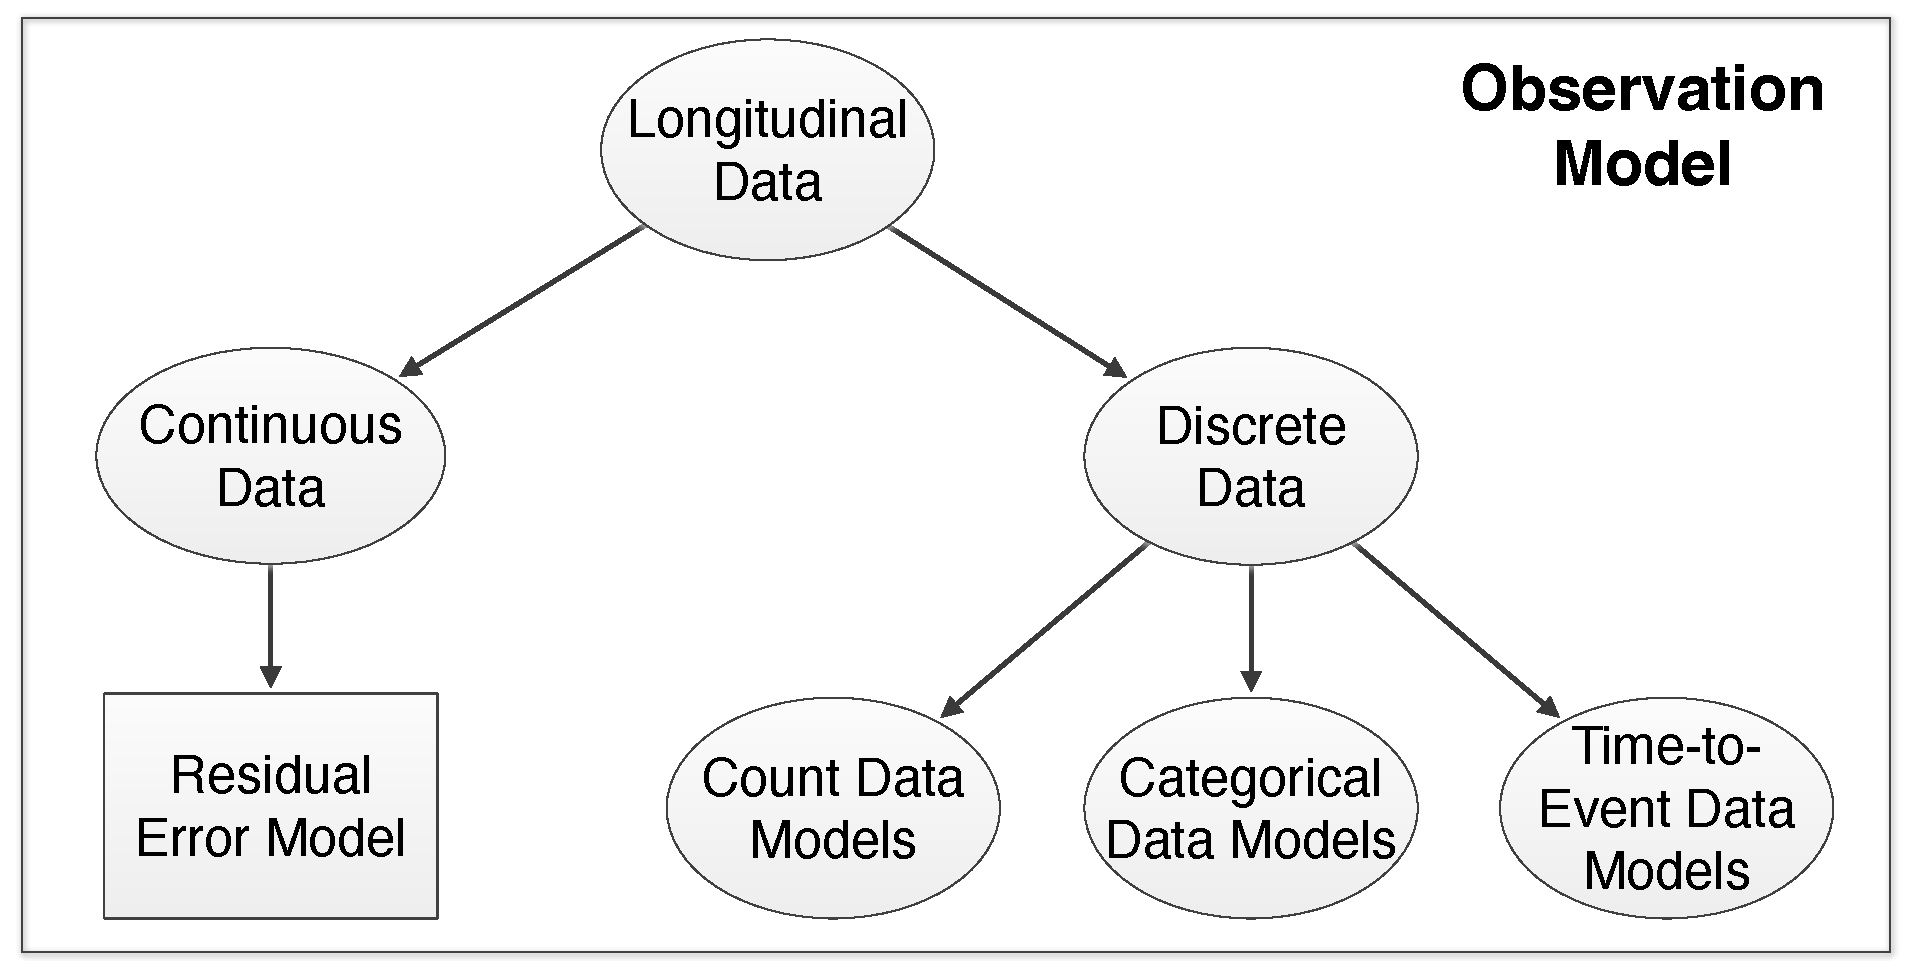
\includegraphics[height=75mm]{pics/observationalModel}
\caption{Observation model for continuous and discrete data. 
The residual error model of continuous data is described by a continuous distribution 
(e.g. normal distribution), while the error distribution of discrete data
is described by a discrete distribution (e.g. binomial for binary data).}
\label{fig:observModel}
\end{figure}


%%%%%%%%%%%%%%%%%%%%%%%%%%%%%%%%%%%%%%%%%%%%%%%%%%%%%%%%%%%%%%%%%%
\subsection{Contiuous data}
\label{subsec:ContinuesData}

An essential component of the continuous observation model is the residual error model.

%%%%%%%%%%%%%%%%%%%%%%%%%%%%%%%%%%%%%%%%%%%%%%%%%%%%%%%%%%%%%%%%%%
\subsubsection{Residual error model}
\label{sec:residualErrorModel}
\label{maths:error_model}
\label{maths:combined-err-model}
In this section we consider different forms of the residual error, i.e. this section is about $g$ in the term
\begin{align*}
g(x_{ij}, \psi_{i}, \xi) \epsilon_{ij}
\end{align*}
of eq.\ref{eq:nlmeModel} with $\epsilon_{ij} \sim N(0, 1)$, i.e. a standard normally distributed random variable. We distinguish between
\begin{itemize}\addtolength{\itemsep}{-.95\baselineskip}
\item
models for \textbf{untransformed} data
\begin{align*}
 \underbrace{ y_{ij}}_{\text{\parbox{2cm}{\centering Experimental \\[-4pt]  data}}} =
 \underbrace{ f(x_{ij}, \psi_{i})}_{\text{\parbox{2.5cm}{\centering Model \\[-4pt]  prediction}}} +
 \underbrace{ g(x_{ij}, \psi_{i}, \xi_i) \; \epsilon_{ij}}_{\text{\parbox{3cm}{\centering Residual \\[-4pt] error}}}
 \end{align*}
 \item
\textbf{transform-both-sides} models
\begin{eqnarray}
 \underbrace{ u(y_{ij})}_{\text{\parbox{2cm}{\centering Transformed \\[-4pt] experimental \\[-4pt]  data}}} =
 \underbrace{ u\big(f(x_{ij}, \psi_{i})\big)}_{\text{\parbox{2.5cm}{\centering Transformed \\[-4pt]  model \\[-4pt]  prediction}}} +
 \underbrace{ g(x_{ij}, \psi_{i}, \xi_i) \; \epsilon_{ij}}_{\text{\parbox{3cm}{\centering Residual \\[-4pt] error}}} \nonumber
 \end{eqnarray}
 \item
and \textbf{implicit} models
\begin{eqnarray}
 \underbrace{ u(y_{ij})}_{\text{\parbox{2.5cm}{\centering Transformed \\[-4pt] experimental  data}}} =
 \underbrace{ U\big(f(x_{ij}, \psi_{i}),\xi_i, \epsilon_{1,ij}, \epsilon_{2,ij}, \dots\big)}_{\text{\parbox{2.5cm}{\centering Transformed \\[-4pt]  model prediction}}} \nonumber
 \end{eqnarray}
\end{itemize}
The \textit{untransformed} form is a special case of the \textit{transform-both-sides} form with $u \equiv Id$, i.e. the identity transformation.
Then for models of both types with $\epsilon_{ij}$ being normally distributed with mean 0 and variance 1, $u(y_{ij})$ is also normally distributed
with mean $u(f(x_{ij}, \psi_{i}))$ and the standard deviation $g(x_{ij}, \psi_{i}, \xi_i)$. \\
Possible extensions to the basic models are
\begin{itemize}
\item
when more than one random variable is applied, i.e. multiple $\epsilon$'s,
\item
when more than one type of measurement or observation is defined, or
\item
when variability, as discussed in section \ref{sec:variabilityModel}, is applied to parameters of the residual error model (see section \ref{subsec:varModelResidualError} for details).
\end{itemize}


%%%%%%%%%%%%%%%%%%%%%%%%%%%%%%%%%%%%%%%%%%%%%%%%%%%%%%%%%%%%%%%%%%
\subsubsection{Incorporating variability on the residual error model parameters}
\label{subsec:varModelResidualError}
In analogy to the nested hierarchical structure for the variability on the individual parameters,
variability on residual error model parameters can be defined using the same structure.
By doing so, no new structure is necessary to account for any inter-individual and/or inter-occasion variability of the residual error model parameters.

This allows \pharmml to cover the so-called 'ETA-on-EPS' approach -- e.g. IIV on the residual error model parameters or in other words varying residual
error magnitude between individuals, see Figure \ref{fig:IOV0_residualError}.
For example, if an additive residual error model and a log-normal distribution for $a$ is assumed, then the parameter model reads
\begin{align*}
	& \log(a_i) = \log(a_{pop}) + \eta_a, \quad  \eta_a \sim \mathcal{N}(0,\omega_a^2)
\end{align*}
and the observation model reads
\begin{align*}
	& y_{ij} \sim \mathcal{N}(f_{ij},a_i^2): \quad y_{ij} = f_{ij} + a_i \epsilon_{ij}, \quad \epsilon_{ij} \sim \mathcal{N}(0,1).
\end{align*}
\begin{figure}[htb!]
\centering
  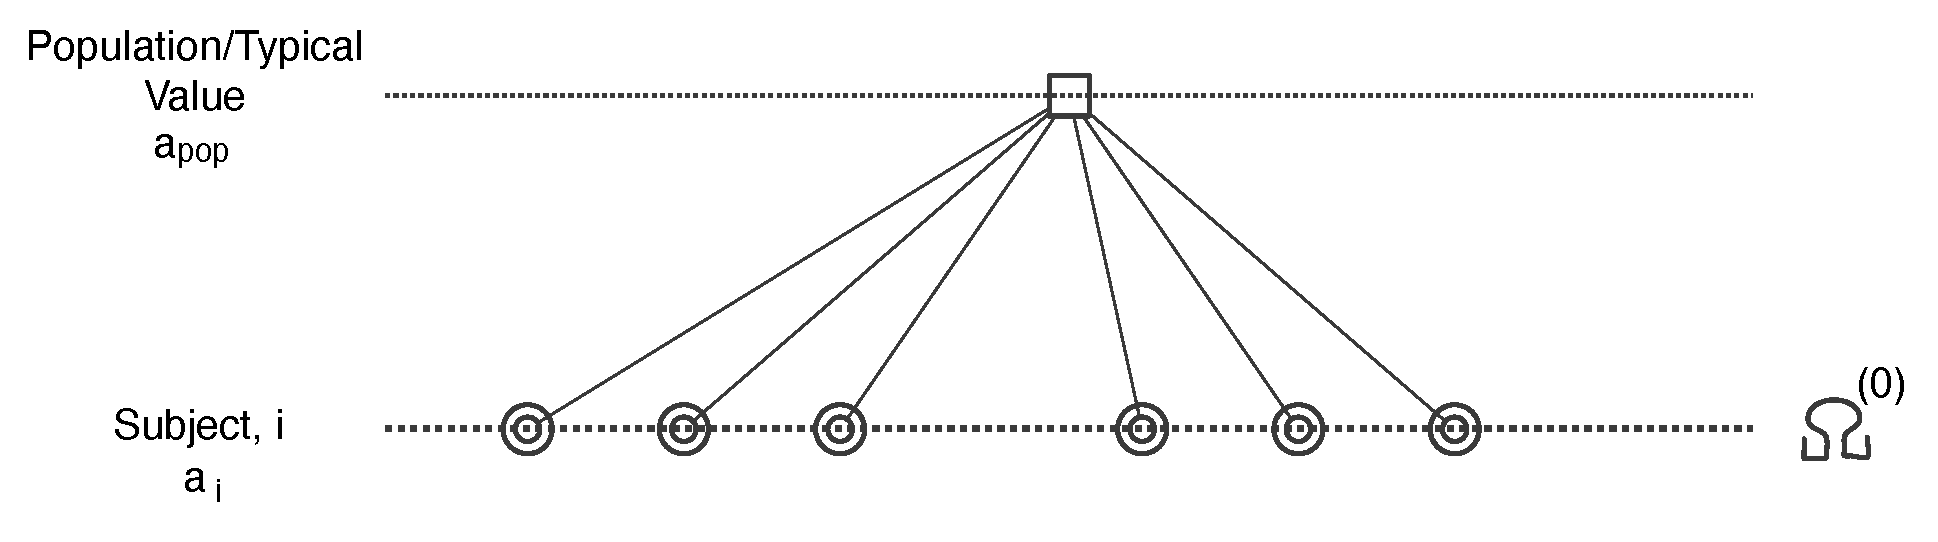
\includegraphics[width=130mm]{pics/IOV0}
 \caption{Inter-individual variability of the residual error parameter $a$. The nested hierarchical structure is identical to that of structural model parameters.}
 \label{fig:IOV0_residualError}
\end{figure}


%%%%%%%%%%%%%%%%%%%%%%%%%%%%%%%%%%%%%%%%%%%%%%%%%%%%%%%%%%%%%%%%%%
\subsubsection{Residual error model examples}
\label{subsec:modelExamples}
Currently, there is no library of residual error models but this might change in the future. All of the following residual error model examples and their different versions can be implemented in the present version of PharmML:
\begin{itemize}
\item
Constant/additive:
\begin{align*}
& y_{ij} = f_{ij} + a \; \epsilon_{ij}; \quad \epsilon_{ij} \sim N(0,1)  \\
\text{or} \quad & y_{ij} = f_{ij} + \epsilon_{ij}; \quad \epsilon_{ij} \sim N(0,\sigma^2)
\end{align*}
\item
Proportional or constant CV (CCV):
\begin{align*}
&y_{ij} =  f_{ij} + bf_{ij} \; \epsilon_{ij}; \quad \epsilon_{ij} \sim N(0,1)  \\
\text{or} \quad & y_{ij} =  f_{ij}(1+\epsilon_{ij}); \quad \epsilon_{ij} \sim N(0,\sigma^2)
\end{align*}
\item
Combined additive and proportional 1:
\begin{align*}
& y_{ij} =  f_{ij} + (a + bf_{ij}) \; \epsilon_{ij}; \quad \epsilon_{ij} \sim N(0,1)
\end{align*}
\item
Combined additive and proportional 2:
\begin{align*}
& y_{ij} =  f_{ij} + \sqrt{a^2 + b^2f_{ij}^2} \; \epsilon_{ij}; \quad \epsilon_{ij} \sim N(0,1)  \\
\text{or}  \quad & y_{ij} =  f_{ij} +  a\, \epsilon_{1,ij} + b f_{ij}\, \epsilon_{2,ij}; \quad \epsilon_{1,ij} \sim N(0,1); \quad \epsilon_{2,ij} \sim N(0,1);   \\
\text{or}  \quad & y_{ij} =  f_{ij} (1 + \epsilon_{1,ij}) + \epsilon_{2,ij}; \quad \epsilon_{1,ij} \sim N(0,\sigma_1^2); \quad \epsilon_{2,ij} \sim N(0,\sigma_2^2);
\end{align*}
\item
Power error model:
\begin{align*}
& y_{ij} = f_{ij} + b\,f_{ij}^c \; \epsilon_{ij}; \quad \epsilon_{ij} \sim N(0,1)
\end{align*}
\item
Combined additive and power error model 1:
\begin{align*}
& y_{ij} =  f_{ij} + (a + b f_{ij}^c) \; \epsilon_{ij}; \quad \epsilon_{ij} \sim N(0,1)
\end{align*}
\item
Combined additive and power error model 2:
\begin{align*}
& y_{ij} = f_{ij} + a\epsilon_{1,ij} + b f_{ij}^c \epsilon_{2,ij}; \quad \epsilon_{1,ij} \sim N(0,1); \quad \epsilon_{2,ij} \sim N(0,1)
\end{align*}
\item
Two (or more) types of measurements error model:
\begin{align*}
& y_{ij} = f_{ij} + \text{ASY}_j\epsilon_{1,ij} + (1-\text{ASY}_j) \epsilon_{2,ij}; \quad \epsilon_{1,ij} \sim N(0,\sigma_1^2); \quad \epsilon_{2,ij} \sim N(0,\sigma_2^2)
\end{align*}
\item
Two (or more) types of observations error model:
\begin{align*}
& y_{ij} = \text{TYP}_{ij} f_{1,ij} + (1-\text{TYP}_{ij}) f_{2,ij} + \text{TYP}_{ij}\epsilon_{1,ij} + (1-\text{TYP}_{ij}) \epsilon_{2,ij};  \\
&  \epsilon_{1,ij} \sim N(0,\sigma_1^2); \quad \epsilon_{2,ij} \sim N(0,\sigma_2^2)
\end{align*}
%\item
%Extended error model:
%
%y_{ij} = \left\{ \begin{array}{rcl}  f_{ij} + \epsilon_{1,ij}  & \mbox{for} & \text{TIME == 1 \&\& ID == 1} \\
%f_{ij} + \epsilon_{2,ij}  & \mbox{for} & \text{TIME == 2 \&\& ID == 1} \\
%\cdots \end{array}\right\} \quad \text{with} \quad
%\epsilon_{1,ij} \sim N(0,\sigma_1^2),\, \epsilon_{2,ij} \sim N(0,\sigma_2^2), \cdots
%
\end{itemize}
Main sources: \cite{NONMEM:2006aa} and \cite{POPIX:2013}.

\subparagraph{Note 1}
In the list above models are pulled together which have the same variance function.
\subparagraph{Note 2}
Models listed above are the most popular ones in use but the present PharmML 
structure allows for implementation of virtually any user-defined model. See 
section ref:XYZ for more examples and PharmML implementation.

%%%%%%%%%%%%%%%%%%%%%%%%%%%%%%%%%%%%%%%%%%%%%%%%%%%%%%%%%%%%%%%%%%
\subsection{Discrete data }
\label{subsec:DiscreteData}

The central piece of information to be provided when modeling discrete data is 
their distribution. While it is possible to encode in PharmML virtually any 
probability mass or density function explicitly, in few cases we can use the UncertML 
\cite{uncertml3:2014} and its extensive collection of distributions. 

The following sections are about the minimal information necessary to be 
implemented for most common types of discrete data models. It is important to note 
that we tried to stay generic rather then to provide the support for 
encoding of models in a particular tool. 

%%%%%%%%%%%%%%%%%%%%%%%%%%%%%%%%%%%%%%%%%%%%%%%%%%%%%%%%%%%%%%%%%%%%
\subsubsection{Count data}
\label{subsec:mmCountData}
An example for count data is the number of events of certain types, such as seizures, heart attacks and 
is typically modelled by the Poisson distribution. In the case of so called \textit{over-dispersed} 
data, i.e. when the variability is greater then what one would expect based on typical data sample, 
we have to resort to more complex models, such as negative binomial or zero-inflated Poisson model, 
see \ref{subsubsec:alternatives}.
Typically the minimal information to be provided consists of:
\begin{itemize}
\item
Type of observed variable -- discrete/count
\item
Count variable, e.g. $y$
\item
Parameters (see also Table \ref{tab:countDataModels})
\begin{itemize}
\item
Rate parameter $\lambda$, also called the Poisson 'intensity' $\lambda_{ij} = \lambda(t_{ij}, \psi_{ij})$, can be
\begin{itemize} %\addtolength{\itemsep}{-.95\baselineskip} 
\item
constant (\emph{homogenous Poisson process})
\begin{eqnarray}
\lambda(t_{ij}, \psi_{i}) = \lambda_{i} \nonumber
\end{eqnarray}
\item
a function of time (\emph{non-homogenous Poisson process})
\begin{eqnarray}
\lambda(t_{ij}, \psi_{i}) = \lambda_{0,i} + a_i t_{ij} \nonumber
\end{eqnarray}
\item
a function of additional regression variables, e.g. drug concentration linked to $\lambda$ via an Imax-model
\begin{eqnarray}
\lambda(t_{ij}, \psi_{i}) = \lambda_{0,i} \Big(1 - Imax_i \frac{C_i(t_{ij})}{IC_{50,i} + C_i(t_{ij})} \Big) \nonumber
\end{eqnarray}
\end{itemize}
\item
Overdispersion parameter, $\tau$ (NB model) %, section \ref{subsec:NBmodel})
\item
Dispersion parameter, $\delta$ (GP model) %, section \ref{subsec:GPmodel})
\item
Mixture probability, $\pi$ (PMIX$_2$ model) %, section \ref{subsec:PMIX2model})
\item
Zero probability, $p_0$ (ZIP model) %, section \ref{subsec:ZIPmodel})
\end{itemize}
\item
Probability mass function (PMF) with a link function. 
For example one can define 
\begin{itemize}
\item
the untransformed PMF, e.g.
\begin{eqnarray}
&& P(y_{ij}=k; \lambda) = \frac{\lambda^k \exp(-\lambda))}{k!} \nonumber
 \end{eqnarray}
\item
or log(Poisson-PMF) 
\begin{eqnarray}
&&	\log(P(y_{ij}=k;\lambda)) = -\lambda + k \log(\lambda) - \log(k!) \nonumber
\end{eqnarray}
%\item
%or explicit PMF definition
%\begin{itemize}
%\item
%PM -- Poisson -- parameter: $\lambda$
%\item
%ZIP -- Zero-inflated Poisson  -- parameters: $\lambda, p_0$
%\item
%GP -- Generalised Poisson -- parameters: $\lambda, \delta$
%\item
%PMIX -- Poisson with mixture distribution -- parameters: $\lambda_1,\lambda_2,\pi$
%\item
%NB -- Negative Binomial -- parameters: $\lambda, \tau$
%\end{itemize}
\end{itemize}
\item
Link function -- one from the list: $\{$\emph{identity}, \emph{log}, \emph{logit}, \emph{probit}$\}$. 
\item
Markovian dependence, see Sec.\ref{subsec:markovian}.
\end{itemize}


The following table gives an overview of common count data models encodable 
in \pharmml.

\begin{table}[htdp]
\centering  % centering table
\begin{tabular}{c c c c c}  
\hline\hline
Short  & Full Model 	& Distribution 	& Dependance 		& Markov \\ [-0.5ex]   
name  & 			& parameters 	& 			 	& order 	\\ [0.5ex]   
\hline
\multicolumn{5}{c}{equi-dispersed data}  \\[.1ex]
\hline
PS  		& Poisson 		& $\lambda$ 	& -- 		& -- 			 \\ [1ex] % & \textsection\ref{subsec:PMmodel} \\ [1ex]
PMAK 	& Poisson with 		& $\lambda_i$ 	& Markov 	& any order 	 \\ [-.5ex] % & \textsection\ref{subsec:PMAKmodel} \\[-.5ex]
		& Markov elements	&			&		& is supported \\[1ex]
\hline
\multicolumn{5}{c}{over-dispersed data}  \\[.1ex]
\hline
NB 		& Negative Binomial 	&  $\lambda, \tau$ 			& -- 	& -- \\ [1ex] % & \textsection\ref{subsec:NBmodel}
ZIP 		& Zero-Inflated Poisson 	& $\lambda, p_0$ 			& -- 	& -- \\ [1ex] % & \textsection\ref{subsec:ZIPmodel} \\ [1ex]
GP 		& Generalized Poisson 	& $\lambda, \delta$ 			& -- 	& -- \\ [1ex] % & \textsection\ref{subsec:GPmodel} \\ [1ex]
PMIX$_2$ & Poisson with 		& $\lambda_1, \lambda_2, \pi$ & -- 	& --  \\ [1ex] % & \textsection\ref{subsec:PMIX2model} \\[-.5ex]
  		& Mixture Distribution 	&  						&  	&  \\[1ex]
% [1ex] adds vertical space
\hline                          % inserts single-line
\end{tabular}
\caption{Overview of most popular count data models as used in pharmacometrics, based on \cite{Plan:2009fk}.
All of them are encodable in PharmML.}
\label{tab:countDataModels}
\end{table}%


\paragraph{Alternative models} 
\label{subsubsec:alternatives}
Poisson model listed above applies to equi-dispersed data only.
There is a number of alternative models which can handle over-dispersed data. 
Note, that the according PMF or log(PMF) has to be explicitly encoded in PharmML, see \cite{Plan:2009fk}:
\begin{itemize}%\addtolength{\itemsep}{-.95\baselineskip} 
\item
Zero-inflated Poisson model, ZIP
\begin{eqnarray}
P(y_{ij} = k; \lambda, p_0) =  \left\{ \begin{array}{rcl} p_0 + (1-p_0) e^{-\lambda} & \mbox{if} & k = 0 \\ 
(1-p_0)\frac{e^{-\lambda}\lambda^k}{k!} & \mbox{if} & k > 0 \end{array}\right. \nonumber
\end{eqnarray}
with $\lambda > 0$ and $p_0 \in [0,1]$
\item
Generalised Poisson model, GP
\begin{eqnarray}
P(y_{ij} = k; \lambda, \delta) &=& \frac{\lambda (\lambda + k \delta)^{k-1} e^{-\lambda - k\delta}}{k!} \nonumber
\end{eqnarray}
with $\lambda > 0$ and  $\delta \in [0,1]$
\item
Poisson model with mixture distribution, PMIX
\begin{eqnarray}
P(y_{ij} = k;\pi,\lambda_1,\lambda_2) &=& \pi \frac{e^{-\lambda_1} \lambda_1^k}{k!} + (1-\pi) \frac{e^{-\lambda_2} \lambda_2^k}{k!} \nonumber
\end{eqnarray}
with $\lambda_1, \lambda_2 > 0$ and $\pi \in [0,1]$
\item
Negative Binomial model, NB
\begin{eqnarray}
P(y_{ij} = k;\lambda,\tau) &=& \frac{\Gamma \big( k + \frac{1}{\tau} \big)}{k! \times \Gamma \big(\frac{1}{\tau} \big)} \times \Bigg( \frac{1}{1 + \tau \times \lambda} \Bigg)^{\frac{1}{\tau}} \times \Bigg(\frac{\lambda}{\frac{1}{\tau} + \lambda} \Bigg)^k \nonumber
\end{eqnarray}
with $\lambda, \tau > 0$.
%\item
%Poisson model with Markovian dependence, PMAK
%\begin{align}
% \lambda = \left\{ \begin{array}{rcl}
%			\lambda_1 & \mbox{for} & yp = 0 \\
%			\lambda_2 & \mbox{for} & yp \neq 0 \nonumber
%\end{array}\right. 
%\quad \text{and} \quad P(y=k; \lambda) = \frac{\lambda^k \exp(-\lambda)}{k!} \nonumber
%\end{align}
\end{itemize}

\subparagraph{Note 1} PharmML 0.4 supports the mathematical functions \textit{gammaln} 
-- logarithm of gamma function and \textit{factln} -- logarithm of the factorial.
\subparagraph{Note 2} Currently only the Poisson distribution is supported by UncertML, 
meaning that all other PMF's have to be implemented explicitly. The Negative Binomial distribution
is featured in UncertML as well but is using a different parametrisation and therefore cannot be used 
for our purposes.

%%%%%%%%%%%%%%%%%%%%%%%%%%%%%%%%%%%%%%%%%%%%%%%%%%%%%%%%%%%%%%%%%%%%
\subsubsection{Categorical data}
\label{subsec:mmCategoricalData}
The standard count data models, as presented in the previous section, are simpler to categorise 
and implement then the categorical ones. This is because for the former the definition of a probability 
mass function (PMF) and few parameters is sufficient. On the contrary the categorical models come 
with a vast variety of probability expressions, such as basic nominal and ordered models but also 
more complex once e.g. adjacent category models, continuation ratio 
models, latent continuous variable model and others. \cite{Paule:2012fk} provides an excellent 
overview of discrete models as used in pharmacodynamics.

Categorical model type deals with data organised in nominal (e.g. presence/absence of an event) 
or ordered (e.g. pain scale) categories. In the first case the probability for each category is defined. 
For the second case the cumulative or tail probabilities have to be defined. Furthermore, there are cases
when Markovian dependency and initial/conditional probabilities have to be considered.

Typically the minimal information to be provided consists of:
\begin{itemize}
\item
Nominal categorical data 
\begin{itemize}
\item
Set of categories, e.g. $\{0,1\}$ or $\{1,2,3\}$
\item
Category variable: e.g. $Y$
\item
Probability for each category
\begin{itemize}
\item
Binomial distribution, e.g. $P(Y=1) = p$ (for $Y \in \{0,1\}$) 
\item
Probabilities for the $k$ (or $k-1$) categories, here for $Y \in \{1,2,3\}$, 
\begin{eqnarray}
&&P(Y=1)=a1/(a1+a2+a3) \nonumber \\
&&P(Y=2)=a2/(a1+a2+a3)  \nonumber \\
&&P(Y=3)=1-P(Y=1)-P(Y=2) \nonumber
\end{eqnarray}
\end{itemize}
\item
or alternatively PMF using predefined distributions in UncertML -- available are following distributions: 
bernoulli, binomial, categorical.
\item
Markovian dependence, see Sec.\ref{subsec:markovian}
\item
Link function from the list $\{$\emph{identity}, \emph{log}, \emph{logit}, \emph{probit}$\}$
%\emph{loglog}, \emph{comloglog}--  {\color{red} \scshape{*}}last two link function have been introduced in the 0.4.1 version.\\
%-- ADD definition  {\color{red} \scshape{*}}\\
\end{itemize}
\item
Ordered categorical data
\begin{itemize}
\item
Set of categories, e.g. $\{0,1\}$ or $\{1,2,3\}$
\item
Category variable: e.g. $Y$
\item
Link function -- one from the list: $\{$\emph{identity}, \emph{log}, \emph{logit}, \emph{probit}, \emph{loglog}, \emph{comploglog}$\}$. 
\item
Probability for $k$ or $(k - 1)$ categories -- using one of the link functions. The possible options are 
\begin{itemize}
\item
Exact Cumulative  probability -- P(Y $\leq$ i), log(P(Y $\leq$ i)), logit(P(Y $\leq$ i)), probit(P(Y $\leq$ i)), loglog(P(Y $\leq$ i)), comploglog(P(Y $\leq$ i)) 
\item
Cumulative  probability -- P(Y$<$i), log(P(Y $<$ i)), logit(P(Y $<$ i)), probit(P(Y $<$ i)), loglog(P(Y $<$ i)), comploglog(P(Y $<$ i)), 
\item
Exact Tail probability  -- P(Y $\geq$ i), log(P(Y $\geq$ i)), logit(P(Y $\geq$ i)), probit(P(Y $\geq$ i)), loglog(P(Y $\geq$ i)), comploglog(P(Y $\geq$ i)) 
\item
Tail probability -- P(Y $>$ i), log(P(Y $>$ i)), logit(P(Y $>$ i)), probit(P(Y $>$ i)), loglog(P(Y $>$ i)), comploglog(P(Y $>$ i)) 
\end{itemize}

e.g. 
\begin{itemize}
\item
Cumulative probabilities, e.g. 
\begin{eqnarray}
&&P(Y\leq1)=a1/(a1+a2+a3) \nonumber \\
&&P(Y\leq2)=(a1+a2)/(a1+a2+a3) \nonumber \\
&&P(Y\leq3)=1-P(Y<=2) \nonumber
\end{eqnarray}
\item
Tail probabilities, e.g. 
\begin{eqnarray}
&& P(Y>1)=(a2+a3)/(a1+a2+a3) \nonumber \\
&& P(Y>2)=a3/(a1+a2+a3)  \nonumber \\ 
&& P(Y>3)=1-P(Y>2) \nonumber
\end{eqnarray}
\item
Cumulative logit probabilities, e.g. 
\begin{align}
& \text{logit}(P(Y\leq1))= \theta_1  \nonumber \\
& \text{logit}(P(Y\leq2))= \theta_1+\theta_2  \nonumber \\
& \text{logit}(P(Y\leq3))=1  \nonumber
\end{align}
\end{itemize}
\item
Markovian dependence, see Sec.\ref{subsec:markovian} for definition and examples.
\end{itemize}
\end{itemize}

\paragraph{Complex categorical data} The proposed PharmML structure allows to encode 
other popular models useful in pharmacometrics \cite{Dobson:2002uq}, for example
\begin{itemize}
\item
Complementary log-log models
\begin{align}
& \log\{-\log[P(y=j)]\} = \beta_0 + \beta_1 x \nonumber
\end{align}
\item
Continuation ratio model
\begin{align}
& \text{logit}\Big[\frac{P(y=j) }{ \sum_{i =j+1}^{J} P(y=i) } \Big] = b + \sum_{j = 1}^{N} \beta_j x_j \nonumber
\end{align}
\item
Adjacent category logit model
\begin{align}
& \log\Big[\frac{P(y=j) }{ P(y=j+1) } \Big] = \sum_{j = 1}^{N} \beta_j x_j \nonumber
\end{align}
\item
Complex logit functions (based on \cite{Girard:1998fk})
\begin{align}
& \log \Big[\frac{P(n_j=r | n_{j-1}=q) }{ 1 - \sum_{j\in \{0,2\}} P(n_j=k | n_{j-1} = q)} \Big] = p_{rqkq} \nonumber
\end{align}
\end{itemize}


%\paragraph{Build-in categorical models} Even though such complex models as shown above are implementable
%explicitly in \pml 
%\cite{Dobson:2002uq}, for example
%\begin{itemize}
%\item
%
%\item
%
%\end{itemize}


%%%%%%%%%%%%%%%%%%%%%%%%%%%%%%%%%%%%%%%%%%%%%%%%%%%%%%%%%%%%%%%%%%%%
\subsubsection{Time-to-event data}
In this case the observation is time until an event occurs, which can be unique or repeated.
The model is fully described by defining the the survival or hazard function. Following minimal information 
needs to provided to ensure lossless encoding of this model type.
\begin{itemize}
\item
Type of observed variable -- discrete/time-to-event
\item
One of the probability distribution defining functions
\begin{itemize}
\item
Hazard function, $h(t; \psi_i)$ or
\item
Survival function $S(t;\psi_i)$
\end{itemize}
\item
Type of censoring
\begin{itemize}
\item
Right censoring -- right censoring time 
\item
Interval censoring -- interval length
\end{itemize}
\item
Maximum number of possible events.
\end{itemize}


%%%%%%%%%%%%%%%%%%%%%%%%%%%%%%%%%%%%%%%%%%%%%%%%%%%%%%%%%%%%%%%%%%%%
\subsubsection{Markovian dependence}
\label{subsec:markovian}

%\begin{figure}[htb!]
%\centering
%  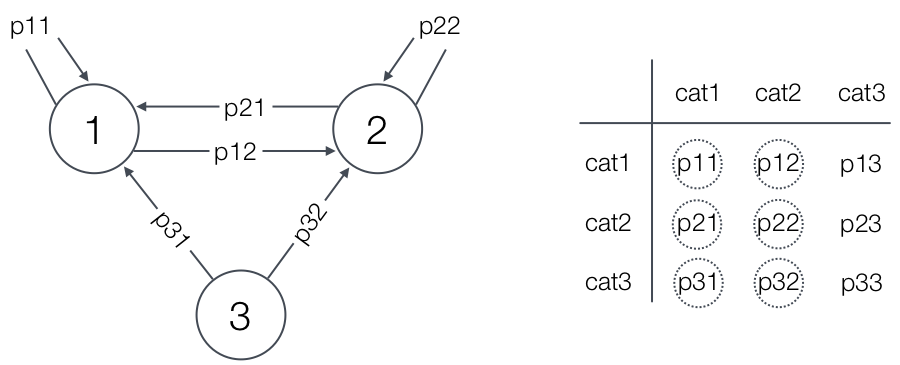
\includegraphics[width=105mm]{pics/markovDependency}
% \caption{An example for Markovian dependence state network.}
% \label{fig:markovDependency}
%\end{figure}
%

To define Markovian dependence in any of those models above, one needs to specify:
\begin{itemize}
\item
State variables as one of the following
\begin{itemize}
\item
Initial state variable, $yinit$
\item
Current state variable, $y$
\item
Previous state variable, $yp$
\end{itemize}
\item
Probability transitions or their alternative transformed forms for a discrete-time models Markov process, e.g.
\begin{align}
& \text{logit}(P(y<=1 | yp=1)) = a11 \nonumber \\
& \text{logit}(P(y<=2 | yp=1)) = a11 + a12\nonumber
\end{align}
with $y$ -- current state, $yp$ -- previous state.
\item
Transition rates for a continuous-time Markov process, \cite{LavielleBook:2014}, e.g.
\begin{align}
& \rho_{1,2}(t) = \exp(a_i+b_i t)  \nonumber \\
& \rho_{2,1}(t) = \exp(c_i+d_i t) \nonumber 
\end{align}
\item
Probability distribution of the initial states, $yinit1, yinit2, ...$ -- 'distribution of first observations'
% -- is equal to the row vector of the stochastic matrix.
\item
Markov order.
\end{itemize}





